\subsection{Autocorrelation of the Active periods in Global View - Results} \label{sec:autocorrelation_active_results}

\subsubsection{Session Experiment - Results} \label{subsec:autocorrelation_sessions}
This experiment will study the session level influence in the independence of the active samples. Following a similar procedure as the one followed in Section \ref{sec:gv_session_exp}, we used different number of sessions but in this case with similar load and studied the autocorrelation function of the active samples of each one of the cases. The flow level (size, interarrival) configuration is fixed and we randomized the packet level with the following configuration:

\begin{itemize}
\item Packet Size distribution: A uniform packet distribution with a normal average [e.g. 1550 bytes] for all flows and for all sessions.
\item An exponential packet inter-arrival time distribution with some practical mean [e.g. 100 ms] for all flows and for all sessions.
\end{itemize}

The final configuration for the different levels of the Extended Multi-Layer traffic model is presented in Table \ref{tab:traffic_autocorrelation_active_gv}:

\begin{table}[h!]
	\begin{center}
		\begin{tabular}{ l | c | c }
			Modeled Variable & Distribution & Parameters \\ \hline
			Session number	& Fixed & N users arriving at simulator start \\
			Flow inter-arrival & Log-normal [Fixed] & $\mu = -1.6355$, $\sigma = 2.6286$ \\
			Flow number & Fixed & Different number depending on desired load \\
			Flow Size & Bi-Pareto [Fixed] & $\alpha = 0.00$, $\beta = 1.02$, $c = 15.56$, $k = 111$ \\
			Packet Size & Uniform & $min = 754$, $max = 2346$ \\
			Packet inter-arrival & Exponential & $\lambda = 10$ \\
		\end{tabular}
		\caption{The parameters used for generating traffic according to the model in \cite{Campus-WLAN}.}
		\label{tab:traffic_autocorrelation_active_gv}
	\end{center}
\end{table}

The indepency of the active samples is studied using the autocorrelation function. We have extracted the sequence of active periods from the traffic generated with the extended multi-layer traffic model which contains which stations (\acs{WLAN} users) had sent the active period. We have obtained the autocorrelation from this sequence of stations. These results are represented in Figure \ref{fig:autocorrelation_sessions}.

\begin{figure}[h!]
	\centering
	\subfloat[]{
		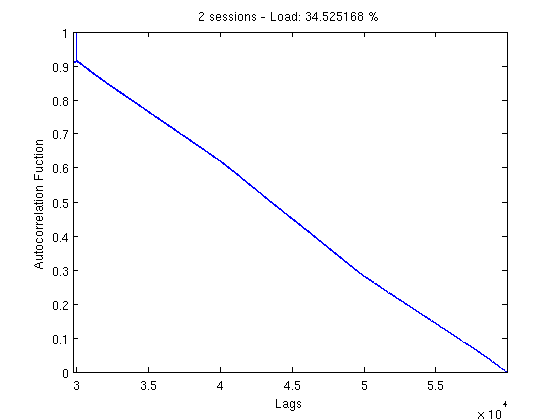
\includegraphics[scale=0.33, trim = 0mm 0mm 0mm 0mm, clip]{images/results/autocorrelation/sessions/2sessions}
		\label{fig:autocorrelation_2sessions}
	}
	\subfloat[]{
		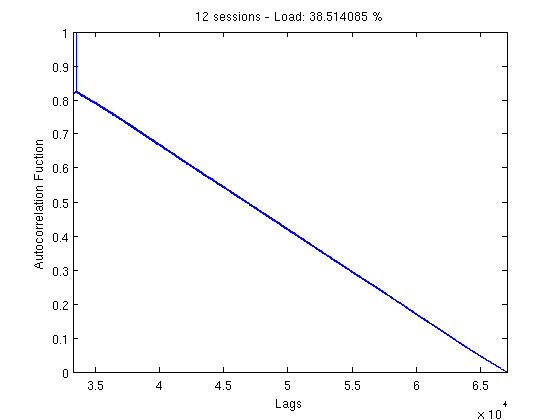
\includegraphics[scale=0.33, trim = 0mm 0mm 0mm 0mm, clip]{images/results/autocorrelation/sessions/12sessions}
		\label{fig:autocorrelation_12sessions}
	}
	\subfloat[]{
		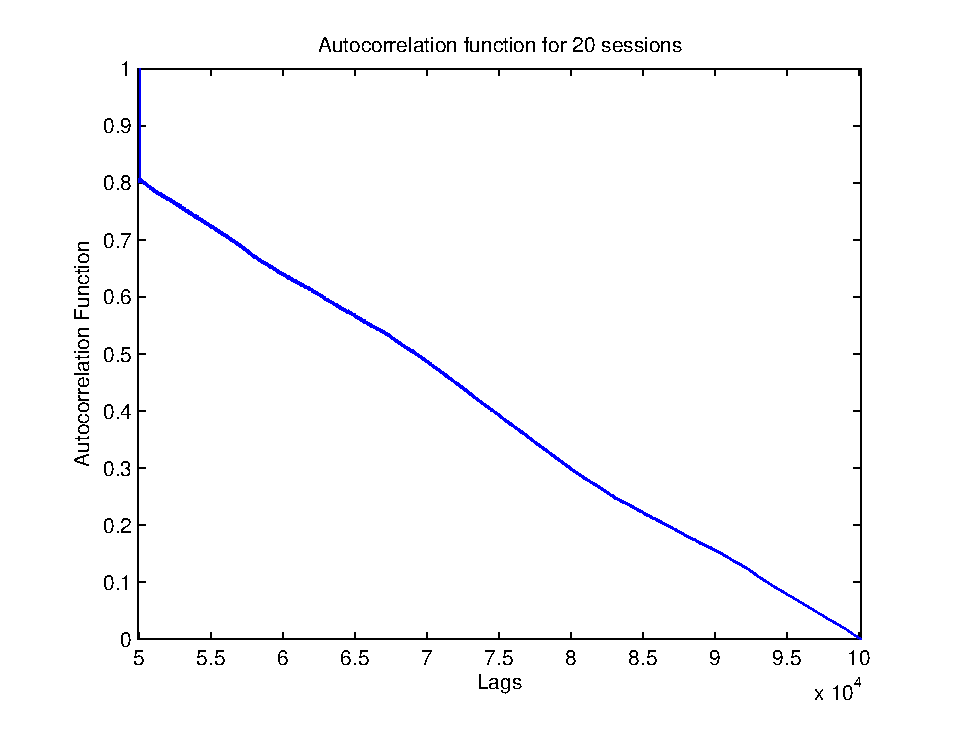
\includegraphics[scale=0.33, trim = 0mm 0mm 0mm 0mm, clip]{images/results/autocorrelation/sessions/20sessions}
		\label{fig:autocorrelation_20sessions}
	}
	\caption{Autocorrelation function for different number of sessions with similar load}
	\label{fig:autocorrelation_sessions}
\end{figure}

In Figure \ref{fig:autocorrelation_sessions} we plotted the autocorrelation function for three different number of sessions cases and similar load in order to compare them. As it can be observed, the higher is the number of sessions, the better is the autocorrelation function. The different harmonics that appear next to the maximum are lower for higher number of sessions. It is clear that the higher is the number of sessions, more random will be the access to the medium of these stations. We can conclude from here then, that the session number improves the autocorrelation properties.

\subsubsection{In-Session Experiment - Results} \label{subsec:autocorrelation_insessions}
Once we tested the effect of the session number in the independence of the sequence of active samples, it is necessary to study how the load affects this independency. In this case, we repeated the experiments using a determined number of sessions (6 \acs{WLAN} users) and we randomized the flow and packet levels and extracted again the autocorrelation function from the stations sequence. The configuration of the different levels of the extended multi-layer traffic model can be found in Table \ref{tab:sim_traffic_model}. The results of this experiment are represented in Figure \ref{fig:autocorrelation_insessions}.

The configuration for the Extended Multi-Layer traffic model is presented in Table \ref{tab:traffic_autocorrelation_active_load_gv}.

\begin{table}[h!]
	\begin{center}
		\begin{tabular}{ l | c | c }
			Modeled Variable & Distribution & Parameters \\ \hline
			Session number	& Fixed & 6 users arriving at simulator start \\
			Flow inter-arrival & Log-normal & $\mu = -1.6355$, $\sigma = 2.6286$ \\
			Flow number & Bi-Pareto & $\alpha = 0.07$, $\beta = 1.75$, $c = 295.38$, $k = 1$ \\
			Flow Size & Bi-Pareto & $\alpha = 0.00$, $\beta = 1.02$, $c = 15.56$, $k = 111$ \\
			Packet Size & Uniform & $min = 754$, $max = 2346$ \\
			Packet inter-arrival & Exponential & $\lambda = 10$ \\
		\end{tabular}
		\caption{The parameters used for generating traffic according to the model in \cite{Campus-WLAN}.}
		\label{tab:traffic_autocorrelation_active_load_gv}
	\end{center}
\end{table}

\begin{figure}[h!]
	\centering
	\subfloat[]{
		\includegraphics[scale=0.33, trim = 0mm 0mm 0mm 0mm, clip]{images/results/autocorrelation/load/36}
		\label{fig:autocorrelation_load36}
	}
	\subfloat[]{
		\includegraphics[scale=0.33, trim = 0mm 0mm 0mm 0mm, clip]{images/results/autocorrelation/load/52}
		\label{fig:autocorrelation_load52}
	}
	\subfloat[]{
		\includegraphics[scale=0.33, trim = 0mm 0mm 0mm 0mm, clip]{images/results/autocorrelation/load/70}
		\label{fig:autocorrelation_load70}
	}
	\caption{Autocorrelation function for load cases}
	\label{fig:autocorrelation_insessions}
\end{figure}

From the results of this experiment, it can be observed that the load clearly affects the autocorrelation function and, in extension, the independence of the samples. For a low load case (Figure \ref{fig:autocorrelation_load36}), the harmonics are clearly present in the autocorrelation function, which means that the samples are not that independent. On the other hand, when the load increases (Figure \ref{fig:autocorrelation_load52}), the harmonics are reduced and finally, when the network is saturated (Figure \ref{fig:autocorrelation_load70}) this harmonics are practically negligible. It can be concluded then, that the increase in the load is translated in a higher independency of the samples. When the network is saturated this independence is almost perfect because of the high random access of the packets to the medium. However, the improvement is not that critical as the one presented in the Session experiment.